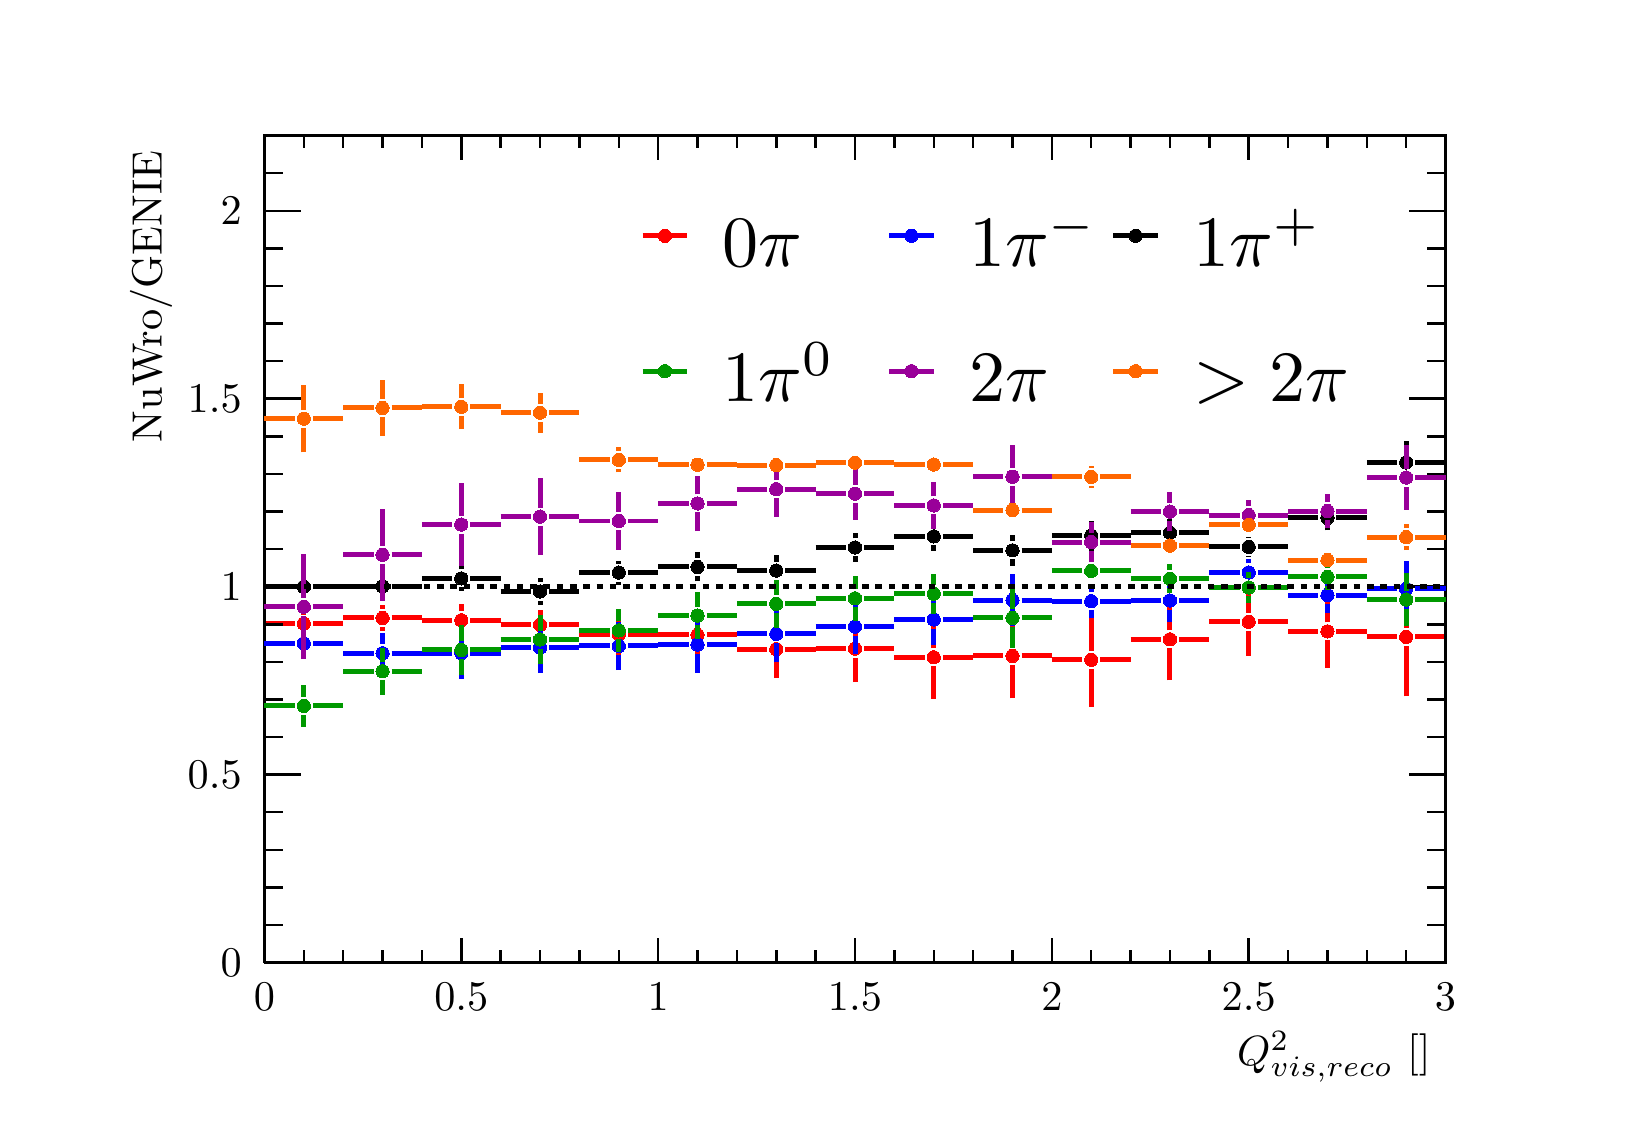
\begin{tikzpicture}
\pgfdeclareplotmark{cross} {
\pgfpathmoveto{\pgfpoint{-0.3\pgfplotmarksize}{\pgfplotmarksize}}
\pgfpathlineto{\pgfpoint{+0.3\pgfplotmarksize}{\pgfplotmarksize}}
\pgfpathlineto{\pgfpoint{+0.3\pgfplotmarksize}{0.3\pgfplotmarksize}}
\pgfpathlineto{\pgfpoint{+1\pgfplotmarksize}{0.3\pgfplotmarksize}}
\pgfpathlineto{\pgfpoint{+1\pgfplotmarksize}{-0.3\pgfplotmarksize}}
\pgfpathlineto{\pgfpoint{+0.3\pgfplotmarksize}{-0.3\pgfplotmarksize}}
\pgfpathlineto{\pgfpoint{+0.3\pgfplotmarksize}{-1.\pgfplotmarksize}}
\pgfpathlineto{\pgfpoint{-0.3\pgfplotmarksize}{-1.\pgfplotmarksize}}
\pgfpathlineto{\pgfpoint{-0.3\pgfplotmarksize}{-0.3\pgfplotmarksize}}
\pgfpathlineto{\pgfpoint{-1.\pgfplotmarksize}{-0.3\pgfplotmarksize}}
\pgfpathlineto{\pgfpoint{-1.\pgfplotmarksize}{0.3\pgfplotmarksize}}
\pgfpathlineto{\pgfpoint{-0.3\pgfplotmarksize}{0.3\pgfplotmarksize}}
\pgfpathclose
\pgfusepathqstroke
}
\pgfdeclareplotmark{cross*} {
\pgfpathmoveto{\pgfpoint{-0.3\pgfplotmarksize}{\pgfplotmarksize}}
\pgfpathlineto{\pgfpoint{+0.3\pgfplotmarksize}{\pgfplotmarksize}}
\pgfpathlineto{\pgfpoint{+0.3\pgfplotmarksize}{0.3\pgfplotmarksize}}
\pgfpathlineto{\pgfpoint{+1\pgfplotmarksize}{0.3\pgfplotmarksize}}
\pgfpathlineto{\pgfpoint{+1\pgfplotmarksize}{-0.3\pgfplotmarksize}}
\pgfpathlineto{\pgfpoint{+0.3\pgfplotmarksize}{-0.3\pgfplotmarksize}}
\pgfpathlineto{\pgfpoint{+0.3\pgfplotmarksize}{-1.\pgfplotmarksize}}
\pgfpathlineto{\pgfpoint{-0.3\pgfplotmarksize}{-1.\pgfplotmarksize}}
\pgfpathlineto{\pgfpoint{-0.3\pgfplotmarksize}{-0.3\pgfplotmarksize}}
\pgfpathlineto{\pgfpoint{-1.\pgfplotmarksize}{-0.3\pgfplotmarksize}}
\pgfpathlineto{\pgfpoint{-1.\pgfplotmarksize}{0.3\pgfplotmarksize}}
\pgfpathlineto{\pgfpoint{-0.3\pgfplotmarksize}{0.3\pgfplotmarksize}}
\pgfpathclose
\pgfusepathqfillstroke
}
\pgfdeclareplotmark{newstar} {
\pgfpathmoveto{\pgfqpoint{0pt}{\pgfplotmarksize}}
\pgfpathlineto{\pgfqpointpolar{44}{0.5\pgfplotmarksize}}
\pgfpathlineto{\pgfqpointpolar{18}{\pgfplotmarksize}}
\pgfpathlineto{\pgfqpointpolar{-20}{0.5\pgfplotmarksize}}
\pgfpathlineto{\pgfqpointpolar{-54}{\pgfplotmarksize}}
\pgfpathlineto{\pgfqpointpolar{-90}{0.5\pgfplotmarksize}}
\pgfpathlineto{\pgfqpointpolar{234}{\pgfplotmarksize}}
\pgfpathlineto{\pgfqpointpolar{198}{0.5\pgfplotmarksize}}
\pgfpathlineto{\pgfqpointpolar{162}{\pgfplotmarksize}}
\pgfpathlineto{\pgfqpointpolar{134}{0.5\pgfplotmarksize}}
\pgfpathclose
\pgfusepathqstroke
}
\pgfdeclareplotmark{newstar*} {
\pgfpathmoveto{\pgfqpoint{0pt}{\pgfplotmarksize}}
\pgfpathlineto{\pgfqpointpolar{44}{0.5\pgfplotmarksize}}
\pgfpathlineto{\pgfqpointpolar{18}{\pgfplotmarksize}}
\pgfpathlineto{\pgfqpointpolar{-20}{0.5\pgfplotmarksize}}
\pgfpathlineto{\pgfqpointpolar{-54}{\pgfplotmarksize}}
\pgfpathlineto{\pgfqpointpolar{-90}{0.5\pgfplotmarksize}}
\pgfpathlineto{\pgfqpointpolar{234}{\pgfplotmarksize}}
\pgfpathlineto{\pgfqpointpolar{198}{0.5\pgfplotmarksize}}
\pgfpathlineto{\pgfqpointpolar{162}{\pgfplotmarksize}}
\pgfpathlineto{\pgfqpointpolar{134}{0.5\pgfplotmarksize}}
\pgfpathclose
\pgfusepathqfillstroke
}
\definecolor{c}{rgb}{1,1,1};
\draw [color=c, fill=c] (0,0) rectangle (20,13.639);
\draw [color=c, fill=c] (3,1.77307) rectangle (18,12.2751);
\definecolor{c}{rgb}{0,0,0};
\draw [c,line width=0.9] (3,1.77307) -- (3,12.2751) -- (18,12.2751) -- (18,1.77307) -- (3,1.77307);
\definecolor{c}{rgb}{1,1,1};
\draw [color=c, fill=c] (3,1.77307) rectangle (18,12.2751);
\definecolor{c}{rgb}{0,0,0};
\draw [c,line width=0.9] (3,1.77307) -- (3,12.2751) -- (18,12.2751) -- (18,1.77307) -- (3,1.77307);
\definecolor{c}{rgb}{1,0,0};
\draw [c,line width=1.8] (3.5,5.91965) -- (3.5,5.96288);
\draw [c,line width=1.8] (3.5,6.1921) -- (3.5,6.23533);
\draw [c,line width=1.8] (3,6.07749) -- (3.38539,6.07749);
\draw [c,line width=1.8] (3.61461,6.07749) -- (4,6.07749);
\foreach \P in {(3.5,6.07749)}{\draw[mark options={color=c,fill=c},mark size=2.402402pt, line width=0.000000pt, mark=*] plot coordinates {\P};}
\draw [c,line width=1.8] (4.5,5.9834) -- (4.5,6.0344);
\draw [c,line width=1.8] (4.5,6.26362) -- (4.5,6.31462);
\draw [c,line width=1.8] (4,6.14901) -- (4.38539,6.14901);
\draw [c,line width=1.8] (4.61461,6.14901) -- (5,6.14901);
\foreach \P in {(4.5,6.14901)}{\draw[mark options={color=c,fill=c},mark size=2.402402pt, line width=0.000000pt, mark=*] plot coordinates {\P};}
\draw [c,line width=1.8] (5.5,5.91648) -- (5.5,6.00588);
\draw [c,line width=1.8] (5.5,6.2351) -- (5.5,6.3245);
\draw [c,line width=1.8] (5,6.12049) -- (5.38539,6.12049);
\draw [c,line width=1.8] (5.61461,6.12049) -- (6,6.12049);
\foreach \P in {(5.5,6.12049)}{\draw[mark options={color=c,fill=c},mark size=2.402402pt, line width=0.000000pt, mark=*] plot coordinates {\P};}
\draw [c,line width=1.8] (6.5,5.87941) -- (6.5,5.94782);
\draw [c,line width=1.8] (6.5,6.17705) -- (6.5,6.24546);
\draw [c,line width=1.8] (6,6.06243) -- (6.38539,6.06243);
\draw [c,line width=1.8] (6.61461,6.06243) -- (7,6.06243);
\foreach \P in {(6.5,6.06243)}{\draw[mark options={color=c,fill=c},mark size=2.402402pt, line width=0.000000pt, mark=*] plot coordinates {\P};}
\draw [c,line width=1.8] (7.5,5.66552) -- (7.5,5.82912);
\draw [c,line width=1.8] (7.5,6.05834) -- (7.5,6.22194);
\draw [c,line width=1.8] (7,5.94373) -- (7.38539,5.94373);
\draw [c,line width=1.8] (7.61461,5.94373) -- (8,5.94373);
\foreach \P in {(7.5,5.94373)}{\draw[mark options={color=c,fill=c},mark size=2.402402pt, line width=0.000000pt, mark=*] plot coordinates {\P};}
\draw [c,line width=1.8] (8.5,5.63415) -- (8.5,5.81865);
\draw [c,line width=1.8] (8.5,6.04787) -- (8.5,6.23237);
\draw [c,line width=1.8] (8,5.93326) -- (8.38539,5.93326);
\draw [c,line width=1.8] (8.61461,5.93326) -- (9,5.93326);
\foreach \P in {(8.5,5.93326)}{\draw[mark options={color=c,fill=c},mark size=2.402402pt, line width=0.000000pt, mark=*] plot coordinates {\P};}
\draw [c,line width=1.8] (9.5,5.38481) -- (9.5,5.63876);
\draw [c,line width=1.8] (9.5,5.86798) -- (9.5,6.12193);
\draw [c,line width=1.8] (9,5.75337) -- (9.38539,5.75337);
\draw [c,line width=1.8] (9.61461,5.75337) -- (10,5.75337);
\foreach \P in {(9.5,5.75337)}{\draw[mark options={color=c,fill=c},mark size=2.402402pt, line width=0.000000pt, mark=*] plot coordinates {\P};}
\draw [c,line width=1.8] (10.5,5.33393) -- (10.5,5.64512);
\draw [c,line width=1.8] (10.5,5.87435) -- (10.5,6.18553);
\draw [c,line width=1.8] (10,5.75973) -- (10.3854,5.75973);
\draw [c,line width=1.8] (10.6146,5.75973) -- (11,5.75973);
\foreach \P in {(10.5,5.75973)}{\draw[mark options={color=c,fill=c},mark size=2.402402pt, line width=0.000000pt, mark=*] plot coordinates {\P};}
\draw [c,line width=1.8] (11.5,5.12056) -- (11.5,5.53551);
\draw [c,line width=1.8] (11.5,5.76474) -- (11.5,6.17968);
\draw [c,line width=1.8] (11,5.65013) -- (11.3854,5.65013);
\draw [c,line width=1.8] (11.6146,5.65013) -- (12,5.65013);
\foreach \P in {(11.5,5.65013)}{\draw[mark options={color=c,fill=c},mark size=2.402402pt, line width=0.000000pt, mark=*] plot coordinates {\P};}
\draw [c,line width=1.8] (12.5,5.12946) -- (12.5,5.55304);
\draw [c,line width=1.8] (12.5,5.78227) -- (12.5,6.20585);
\draw [c,line width=1.8] (12,5.66765) -- (12.3854,5.66765);
\draw [c,line width=1.8] (12.6146,5.66765) -- (13,5.66765);
\foreach \P in {(12.5,5.66765)}{\draw[mark options={color=c,fill=c},mark size=2.402402pt, line width=0.000000pt, mark=*] plot coordinates {\P};}
\draw [c,line width=1.8] (13.5,5.02084) -- (13.5,5.50368);
\draw [c,line width=1.8] (13.5,5.73291) -- (13.5,6.21575);
\draw [c,line width=1.8] (13,5.6183) -- (13.3854,5.6183);
\draw [c,line width=1.8] (13.6146,5.6183) -- (14,5.6183);
\foreach \P in {(13.5,5.6183)}{\draw[mark options={color=c,fill=c},mark size=2.402402pt, line width=0.000000pt, mark=*] plot coordinates {\P};}
\draw [c,line width=1.8] (14.5,5.357) -- (14.5,5.76334);
\draw [c,line width=1.8] (14.5,5.99257) -- (14.5,6.39891);
\draw [c,line width=1.8] (14,5.87796) -- (14.3854,5.87796);
\draw [c,line width=1.8] (14.6146,5.87796) -- (15,5.87796);
\foreach \P in {(14.5,5.87796)}{\draw[mark options={color=c,fill=c},mark size=2.402402pt, line width=0.000000pt, mark=*] plot coordinates {\P};}
\draw [c,line width=1.8] (15.5,5.67001) -- (15.5,5.98588);
\draw [c,line width=1.8] (15.5,6.21511) -- (15.5,6.53098);
\draw [c,line width=1.8] (15,6.1005) -- (15.3854,6.1005);
\draw [c,line width=1.8] (15.6146,6.1005) -- (16,6.1005);
\foreach \P in {(15.5,6.1005)}{\draw[mark options={color=c,fill=c},mark size=2.402402pt, line width=0.000000pt, mark=*] plot coordinates {\P};}
\draw [c,line width=1.8] (16.5,5.51812) -- (16.5,5.86458);
\draw [c,line width=1.8] (16.5,6.0938) -- (16.5,6.44025);
\draw [c,line width=1.8] (16,5.97919) -- (16.3854,5.97919);
\draw [c,line width=1.8] (16.6146,5.97919) -- (17,5.97919);
\foreach \P in {(16.5,5.97919)}{\draw[mark options={color=c,fill=c},mark size=2.402402pt, line width=0.000000pt, mark=*] plot coordinates {\P};}
\draw [c,line width=1.8] (17.5,5.1519) -- (17.5,5.79408);
\draw [c,line width=1.8] (17.5,6.0233) -- (17.5,6.66548);
\draw [c,line width=1.8] (17,5.90869) -- (17.3854,5.90869);
\draw [c,line width=1.8] (17.6146,5.90869) -- (18,5.90869);
\foreach \P in {(17.5,5.90869)}{\draw[mark options={color=c,fill=c},mark size=2.402402pt, line width=0.000000pt, mark=*] plot coordinates {\P};}
\definecolor{c}{rgb}{0,0,0};
\draw [c,line width=0.9] (3,1.77307) -- (18,1.77307);
\draw [c,line width=0.9] (3,2.07994) -- (3,1.77307);
\draw [c,line width=0.9] (3.5,1.9265) -- (3.5,1.77307);
\draw [c,line width=0.9] (4,1.9265) -- (4,1.77307);
\draw [c,line width=0.9] (4.5,1.9265) -- (4.5,1.77307);
\draw [c,line width=0.9] (5,1.9265) -- (5,1.77307);
\draw [c,line width=0.9] (5.5,2.07994) -- (5.5,1.77307);
\draw [c,line width=0.9] (6,1.9265) -- (6,1.77307);
\draw [c,line width=0.9] (6.5,1.9265) -- (6.5,1.77307);
\draw [c,line width=0.9] (7,1.9265) -- (7,1.77307);
\draw [c,line width=0.9] (7.5,1.9265) -- (7.5,1.77307);
\draw [c,line width=0.9] (8,2.07994) -- (8,1.77307);
\draw [c,line width=0.9] (8.5,1.9265) -- (8.5,1.77307);
\draw [c,line width=0.9] (9,1.9265) -- (9,1.77307);
\draw [c,line width=0.9] (9.5,1.9265) -- (9.5,1.77307);
\draw [c,line width=0.9] (10,1.9265) -- (10,1.77307);
\draw [c,line width=0.9] (10.5,2.07994) -- (10.5,1.77307);
\draw [c,line width=0.9] (11,1.9265) -- (11,1.77307);
\draw [c,line width=0.9] (11.5,1.9265) -- (11.5,1.77307);
\draw [c,line width=0.9] (12,1.9265) -- (12,1.77307);
\draw [c,line width=0.9] (12.5,1.9265) -- (12.5,1.77307);
\draw [c,line width=0.9] (13,2.07994) -- (13,1.77307);
\draw [c,line width=0.9] (13.5,1.9265) -- (13.5,1.77307);
\draw [c,line width=0.9] (14,1.9265) -- (14,1.77307);
\draw [c,line width=0.9] (14.5,1.9265) -- (14.5,1.77307);
\draw [c,line width=0.9] (15,1.9265) -- (15,1.77307);
\draw [c,line width=0.9] (15.5,2.07994) -- (15.5,1.77307);
\draw [c,line width=0.9] (16,1.9265) -- (16,1.77307);
\draw [c,line width=0.9] (16.5,1.9265) -- (16.5,1.77307);
\draw [c,line width=0.9] (17,1.9265) -- (17,1.77307);
\draw [c,line width=0.9] (17.5,1.9265) -- (17.5,1.77307);
\draw [c,line width=0.9] (18,2.07994) -- (18,1.77307);
\draw [c,line width=0.9] (18,2.07994) -- (18,1.77307);
\draw [anchor=base] (3,1.15931) node[scale=1.52731, color=c, rotate=0]{0};
\draw [anchor=base] (5.5,1.15931) node[scale=1.52731, color=c, rotate=0]{0.5};
\draw [anchor=base] (8,1.15931) node[scale=1.52731, color=c, rotate=0]{1};
\draw [anchor=base] (10.5,1.15931) node[scale=1.52731, color=c, rotate=0]{1.5};
\draw [anchor=base] (13,1.15931) node[scale=1.52731, color=c, rotate=0]{2};
\draw [anchor=base] (15.5,1.15931) node[scale=1.52731, color=c, rotate=0]{2.5};
\draw [anchor=base] (18,1.15931) node[scale=1.52731, color=c, rotate=0]{3};
\draw [anchor= east] (18,0.572837) node[scale=1.52731, color=c, rotate=0]{$Q^{2}_{\text{vis, reco}}$ [\si{\giga\electronvolt\squared}] };
\draw [c,line width=0.9] (3,12.2751) -- (18,12.2751);
\draw [c,line width=0.9] (3,11.9682) -- (3,12.2751);
\draw [c,line width=0.9] (3.5,12.1216) -- (3.5,12.2751);
\draw [c,line width=0.9] (4,12.1216) -- (4,12.2751);
\draw [c,line width=0.9] (4.5,12.1216) -- (4.5,12.2751);
\draw [c,line width=0.9] (5,12.1216) -- (5,12.2751);
\draw [c,line width=0.9] (5.5,11.9682) -- (5.5,12.2751);
\draw [c,line width=0.9] (6,12.1216) -- (6,12.2751);
\draw [c,line width=0.9] (6.5,12.1216) -- (6.5,12.2751);
\draw [c,line width=0.9] (7,12.1216) -- (7,12.2751);
\draw [c,line width=0.9] (7.5,12.1216) -- (7.5,12.2751);
\draw [c,line width=0.9] (8,11.9682) -- (8,12.2751);
\draw [c,line width=0.9] (8.5,12.1216) -- (8.5,12.2751);
\draw [c,line width=0.9] (9,12.1216) -- (9,12.2751);
\draw [c,line width=0.9] (9.5,12.1216) -- (9.5,12.2751);
\draw [c,line width=0.9] (10,12.1216) -- (10,12.2751);
\draw [c,line width=0.9] (10.5,11.9682) -- (10.5,12.2751);
\draw [c,line width=0.9] (11,12.1216) -- (11,12.2751);
\draw [c,line width=0.9] (11.5,12.1216) -- (11.5,12.2751);
\draw [c,line width=0.9] (12,12.1216) -- (12,12.2751);
\draw [c,line width=0.9] (12.5,12.1216) -- (12.5,12.2751);
\draw [c,line width=0.9] (13,11.9682) -- (13,12.2751);
\draw [c,line width=0.9] (13.5,12.1216) -- (13.5,12.2751);
\draw [c,line width=0.9] (14,12.1216) -- (14,12.2751);
\draw [c,line width=0.9] (14.5,12.1216) -- (14.5,12.2751);
\draw [c,line width=0.9] (15,12.1216) -- (15,12.2751);
\draw [c,line width=0.9] (15.5,11.9682) -- (15.5,12.2751);
\draw [c,line width=0.9] (16,12.1216) -- (16,12.2751);
\draw [c,line width=0.9] (16.5,12.1216) -- (16.5,12.2751);
\draw [c,line width=0.9] (17,12.1216) -- (17,12.2751);
\draw [c,line width=0.9] (17.5,12.1216) -- (17.5,12.2751);
\draw [c,line width=0.9] (18,11.9682) -- (18,12.2751);
\draw [c,line width=0.9] (18,11.9682) -- (18,12.2751);
\draw [c,line width=0.9] (3,1.77307) -- (3,12.2751);
\draw [c,line width=0.9] (3.462,1.77307) -- (3,1.77307);
\draw [c,line width=0.9] (3.231,2.25043) -- (3,2.25043);
\draw [c,line width=0.9] (3.231,2.72779) -- (3,2.72779);
\draw [c,line width=0.9] (3.231,3.20516) -- (3,3.20516);
\draw [c,line width=0.9] (3.231,3.68252) -- (3,3.68252);
\draw [c,line width=0.9] (3.462,4.15989) -- (3,4.15989);
\draw [c,line width=0.9] (3.231,4.63725) -- (3,4.63725);
\draw [c,line width=0.9] (3.231,5.11461) -- (3,5.11461);
\draw [c,line width=0.9] (3.231,5.59198) -- (3,5.59198);
\draw [c,line width=0.9] (3.231,6.06934) -- (3,6.06934);
\draw [c,line width=0.9] (3.462,6.5467) -- (3,6.5467);
\draw [c,line width=0.9] (3.231,7.02407) -- (3,7.02407);
\draw [c,line width=0.9] (3.231,7.50143) -- (3,7.50143);
\draw [c,line width=0.9] (3.231,7.9788) -- (3,7.9788);
\draw [c,line width=0.9] (3.231,8.45616) -- (3,8.45616);
\draw [c,line width=0.9] (3.462,8.93352) -- (3,8.93352);
\draw [c,line width=0.9] (3.231,9.41089) -- (3,9.41089);
\draw [c,line width=0.9] (3.231,9.88825) -- (3,9.88825);
\draw [c,line width=0.9] (3.231,10.3656) -- (3,10.3656);
\draw [c,line width=0.9] (3.231,10.843) -- (3,10.843);
\draw [c,line width=0.9] (3.462,11.3203) -- (3,11.3203);
\draw [c,line width=0.9] (3.462,11.3203) -- (3,11.3203);
\draw [c,line width=0.9] (3.231,11.7977) -- (3,11.7977);
\draw [c,line width=0.9] (3.231,12.2751) -- (3,12.2751);
\draw [anchor= east] (2.9,1.77307) node[scale=1.52731, color=c, rotate=0]{0};
\draw [anchor= east] (2.9,4.15989) node[scale=1.52731, color=c, rotate=0]{0.5};
\draw [anchor= east] (2.9,6.5467) node[scale=1.52731, color=c, rotate=0]{1};
\draw [anchor= east] (2.9,8.93352) node[scale=1.52731, color=c, rotate=0]{1.5};
\draw [anchor= east] (2.9,11.3203) node[scale=1.52731, color=c, rotate=0]{2};
\draw [anchor= east] (1.56,12.2751) node[scale=1.52731, color=c, rotate=90]{ NuWro/GENIE};
\draw [c,line width=0.9] (18,1.77307) -- (18,12.2751);
\draw [c,line width=0.9] (17.538,1.77307) -- (18,1.77307);
\draw [c,line width=0.9] (17.769,2.25043) -- (18,2.25043);
\draw [c,line width=0.9] (17.769,2.72779) -- (18,2.72779);
\draw [c,line width=0.9] (17.769,3.20516) -- (18,3.20516);
\draw [c,line width=0.9] (17.769,3.68252) -- (18,3.68252);
\draw [c,line width=0.9] (17.538,4.15989) -- (18,4.15989);
\draw [c,line width=0.9] (17.769,4.63725) -- (18,4.63725);
\draw [c,line width=0.9] (17.769,5.11461) -- (18,5.11461);
\draw [c,line width=0.9] (17.769,5.59198) -- (18,5.59198);
\draw [c,line width=0.9] (17.769,6.06934) -- (18,6.06934);
\draw [c,line width=0.9] (17.538,6.5467) -- (18,6.5467);
\draw [c,line width=0.9] (17.769,7.02407) -- (18,7.02407);
\draw [c,line width=0.9] (17.769,7.50143) -- (18,7.50143);
\draw [c,line width=0.9] (17.769,7.9788) -- (18,7.9788);
\draw [c,line width=0.9] (17.769,8.45616) -- (18,8.45616);
\draw [c,line width=0.9] (17.538,8.93352) -- (18,8.93352);
\draw [c,line width=0.9] (17.769,9.41089) -- (18,9.41089);
\draw [c,line width=0.9] (17.769,9.88825) -- (18,9.88825);
\draw [c,line width=0.9] (17.769,10.3656) -- (18,10.3656);
\draw [c,line width=0.9] (17.769,10.843) -- (18,10.843);
\draw [c,line width=0.9] (17.538,11.3203) -- (18,11.3203);
\draw [c,line width=0.9] (17.538,11.3203) -- (18,11.3203);
\draw [c,line width=0.9] (17.769,11.7977) -- (18,11.7977);
\draw [c,line width=0.9] (17.769,12.2751) -- (18,12.2751);
\definecolor{c}{rgb}{0,0,1};
\draw [c,line width=1.8] (3.5,5.68139) -- (3.5,5.71133);
\draw [c,line width=1.8] (3.5,5.94056) -- (3.5,5.9705);
\draw [c,line width=1.8] (3,5.82594) -- (3.38539,5.82594);
\draw [c,line width=1.8] (3.61461,5.82594) -- (4,5.82594);
\foreach \P in {(3.5,5.82594)}{\draw[mark options={color=c,fill=c},mark size=2.402402pt, line width=0.000000pt, mark=*] plot coordinates {\P};}
\draw [c,line width=1.8] (4.5,5.44436) -- (4.5,5.58732);
\draw [c,line width=1.8] (4.5,5.81655) -- (4.5,5.95951);
\draw [c,line width=1.8] (4,5.70194) -- (4.38539,5.70194);
\draw [c,line width=1.8] (4.61461,5.70194) -- (5,5.70194);
\foreach \P in {(4.5,5.70194)}{\draw[mark options={color=c,fill=c},mark size=2.402402pt, line width=0.000000pt, mark=*] plot coordinates {\P};}
\draw [c,line width=1.8] (5.5,5.37999) -- (5.5,5.58796);
\draw [c,line width=1.8] (5.5,5.81719) -- (5.5,6.02517);
\draw [c,line width=1.8] (5,5.70258) -- (5.38539,5.70258);
\draw [c,line width=1.8] (5.61461,5.70258) -- (6,5.70258);
\foreach \P in {(5.5,5.70258)}{\draw[mark options={color=c,fill=c},mark size=2.402402pt, line width=0.000000pt, mark=*] plot coordinates {\P};}
\draw [c,line width=1.8] (6.5,5.44931) -- (6.5,5.657);
\draw [c,line width=1.8] (6.5,5.88622) -- (6.5,6.09391);
\draw [c,line width=1.8] (6,5.77161) -- (6.38539,5.77161);
\draw [c,line width=1.8] (6.61461,5.77161) -- (7,5.77161);
\foreach \P in {(6.5,5.77161)}{\draw[mark options={color=c,fill=c},mark size=2.402402pt, line width=0.000000pt, mark=*] plot coordinates {\P};}
\draw [c,line width=1.8] (7.5,5.48606) -- (7.5,5.67883);
\draw [c,line width=1.8] (7.5,5.90805) -- (7.5,6.10082);
\draw [c,line width=1.8] (7,5.79344) -- (7.38539,5.79344);
\draw [c,line width=1.8] (7.61461,5.79344) -- (8,5.79344);
\foreach \P in {(7.5,5.79344)}{\draw[mark options={color=c,fill=c},mark size=2.402402pt, line width=0.000000pt, mark=*] plot coordinates {\P};}
\draw [c,line width=1.8] (8.5,5.45098) -- (8.5,5.69633);
\draw [c,line width=1.8] (8.5,5.92556) -- (8.5,6.17092);
\draw [c,line width=1.8] (8,5.81095) -- (8.38539,5.81095);
\draw [c,line width=1.8] (8.61461,5.81095) -- (9,5.81095);
\foreach \P in {(8.5,5.81095)}{\draw[mark options={color=c,fill=c},mark size=2.402402pt, line width=0.000000pt, mark=*] plot coordinates {\P};}
\draw [c,line width=1.8] (9.5,5.59415) -- (9.5,5.83177);
\draw [c,line width=1.8] (9.5,6.061) -- (9.5,6.29861);
\draw [c,line width=1.8] (9,5.94638) -- (9.38539,5.94638);
\draw [c,line width=1.8] (9.61461,5.94638) -- (10,5.94638);
\foreach \P in {(9.5,5.94638)}{\draw[mark options={color=c,fill=c},mark size=2.402402pt, line width=0.000000pt, mark=*] plot coordinates {\P};}
\draw [c,line width=1.8] (10.5,5.69761) -- (10.5,5.9237);
\draw [c,line width=1.8] (10.5,6.15293) -- (10.5,6.37902);
\draw [c,line width=1.8] (10,6.03831) -- (10.3854,6.03831);
\draw [c,line width=1.8] (10.6146,6.03831) -- (11,6.03831);
\foreach \P in {(10.5,6.03831)}{\draw[mark options={color=c,fill=c},mark size=2.402402pt, line width=0.000000pt, mark=*] plot coordinates {\P};}
\draw [c,line width=1.8] (11.5,5.80946) -- (11.5,6.01525);
\draw [c,line width=1.8] (11.5,6.24447) -- (11.5,6.45026);
\draw [c,line width=1.8] (11,6.12986) -- (11.3854,6.12986);
\draw [c,line width=1.8] (11.6146,6.12986) -- (12,6.12986);
\foreach \P in {(11.5,6.12986)}{\draw[mark options={color=c,fill=c},mark size=2.402402pt, line width=0.000000pt, mark=*] plot coordinates {\P};}
\draw [c,line width=1.8] (12.5,6.04921) -- (12.5,6.26172);
\draw [c,line width=1.8] (12.5,6.49095) -- (12.5,6.70346);
\draw [c,line width=1.8] (12,6.37633) -- (12.3854,6.37633);
\draw [c,line width=1.8] (12.6146,6.37633) -- (13,6.37633);
\foreach \P in {(12.5,6.37633)}{\draw[mark options={color=c,fill=c},mark size=2.402402pt, line width=0.000000pt, mark=*] plot coordinates {\P};}
\draw [c,line width=1.8] (13.5,6.14492) -- (13.5,6.24764);
\draw [c,line width=1.8] (13.5,6.47686) -- (13.5,6.57958);
\draw [c,line width=1.8] (13,6.36225) -- (13.3854,6.36225);
\draw [c,line width=1.8] (13.6146,6.36225) -- (14,6.36225);
\foreach \P in {(13.5,6.36225)}{\draw[mark options={color=c,fill=c},mark size=2.402402pt, line width=0.000000pt, mark=*] plot coordinates {\P};}
\draw [c,line width=1.8] (14.5,6.10108) -- (14.5,6.25625);
\draw [c,line width=1.8] (14.5,6.48548) -- (14.5,6.64066);
\draw [c,line width=1.8] (14,6.37087) -- (14.3854,6.37087);
\draw [c,line width=1.8] (14.6146,6.37087) -- (15,6.37087);
\foreach \P in {(14.5,6.37087)}{\draw[mark options={color=c,fill=c},mark size=2.402402pt, line width=0.000000pt, mark=*] plot coordinates {\P};}
\draw [c,line width=1.8] (15.5,6.55055) -- (15.5,6.61235);
\draw [c,line width=1.8] (15.5,6.84158) -- (15.5,6.90338);
\draw [c,line width=1.8] (15,6.72696) -- (15.3854,6.72696);
\draw [c,line width=1.8] (15.6146,6.72696) -- (16,6.72696);
\foreach \P in {(15.5,6.72696)}{\draw[mark options={color=c,fill=c},mark size=2.402402pt, line width=0.000000pt, mark=*] plot coordinates {\P};}
\draw [c,line width=1.8] (16.5,6.21202) -- (16.5,6.32487);
\draw [c,line width=1.8] (16.5,6.55409) -- (16.5,6.66694);
\draw [c,line width=1.8] (16,6.43948) -- (16.3854,6.43948);
\draw [c,line width=1.8] (16.6146,6.43948) -- (17,6.43948);
\foreach \P in {(16.5,6.43948)}{\draw[mark options={color=c,fill=c},mark size=2.402402pt, line width=0.000000pt, mark=*] plot coordinates {\P};}
\draw [c,line width=1.8] (17.5,6.16779) -- (17.5,6.40526);
\draw [c,line width=1.8] (17.5,6.63449) -- (17.5,6.87196);
\draw [c,line width=1.8] (17,6.51987) -- (17.3854,6.51987);
\draw [c,line width=1.8] (17.6146,6.51987) -- (18,6.51987);
\foreach \P in {(17.5,6.51987)}{\draw[mark options={color=c,fill=c},mark size=2.402402pt, line width=0.000000pt, mark=*] plot coordinates {\P};}
\definecolor{c}{rgb}{0,0,0};
\draw [c,line width=1.8] (3,6.54565) -- (3.38539,6.54565);
\draw [c,line width=1.8] (3.61461,6.54565) -- (4,6.54565);
\foreach \P in {(3.5,6.54565)}{\draw[mark options={color=c,fill=c},mark size=2.402402pt, line width=0.000000pt, mark=*] plot coordinates {\P};}
\draw [c,line width=1.8] (4.5,6.43104) -- (4.5,6.4373);
\draw [c,line width=1.8] (4.5,6.66653) -- (4.5,6.67279);
\draw [c,line width=1.8] (4,6.55191) -- (4.38539,6.55191);
\draw [c,line width=1.8] (4.61461,6.55191) -- (5,6.55191);
\foreach \P in {(4.5,6.55191)}{\draw[mark options={color=c,fill=c},mark size=2.402402pt, line width=0.000000pt, mark=*] plot coordinates {\P};}
\draw [c,line width=1.8] (5.5,6.49715) -- (5.5,6.53704);
\draw [c,line width=1.8] (5.5,6.76627) -- (5.5,6.80617);
\draw [c,line width=1.8] (5,6.65166) -- (5.38539,6.65166);
\draw [c,line width=1.8] (5.61461,6.65166) -- (6,6.65166);
\foreach \P in {(5.5,6.65166)}{\draw[mark options={color=c,fill=c},mark size=2.402402pt, line width=0.000000pt, mark=*] plot coordinates {\P};}
\draw [c,line width=1.8] (6.5,6.31772) -- (6.5,6.3705);
\draw [c,line width=1.8] (6.5,6.59972) -- (6.5,6.6525);
\draw [c,line width=1.8] (6,6.48511) -- (6.38539,6.48511);
\draw [c,line width=1.8] (6.61461,6.48511) -- (7,6.48511);
\foreach \P in {(6.5,6.48511)}{\draw[mark options={color=c,fill=c},mark size=2.402402pt, line width=0.000000pt, mark=*] plot coordinates {\P};}
\draw [c,line width=1.8] (7.5,6.57371) -- (7.5,6.61085);
\draw [c,line width=1.8] (7.5,6.84008) -- (7.5,6.87722);
\draw [c,line width=1.8] (7,6.72547) -- (7.38539,6.72547);
\draw [c,line width=1.8] (7.61461,6.72547) -- (8,6.72547);
\foreach \P in {(7.5,6.72547)}{\draw[mark options={color=c,fill=c},mark size=2.402402pt, line width=0.000000pt, mark=*] plot coordinates {\P};}
\draw [c,line width=1.8] (8.5,6.61443) -- (8.5,6.68362);
\draw [c,line width=1.8] (8.5,6.91285) -- (8.5,6.98204);
\draw [c,line width=1.8] (8,6.79823) -- (8.38539,6.79823);
\draw [c,line width=1.8] (8.61461,6.79823) -- (9,6.79823);
\foreach \P in {(8.5,6.79823)}{\draw[mark options={color=c,fill=c},mark size=2.402402pt, line width=0.000000pt, mark=*] plot coordinates {\P};}
\draw [c,line width=1.8] (9.5,6.557) -- (9.5,6.63622);
\draw [c,line width=1.8] (9.5,6.86545) -- (9.5,6.94467);
\draw [c,line width=1.8] (9,6.75083) -- (9.38539,6.75083);
\draw [c,line width=1.8] (9.61461,6.75083) -- (10,6.75083);
\foreach \P in {(9.5,6.75083)}{\draw[mark options={color=c,fill=c},mark size=2.402402pt, line width=0.000000pt, mark=*] plot coordinates {\P};}
\draw [c,line width=1.8] (10.5,6.86104) -- (10.5,6.92993);
\draw [c,line width=1.8] (10.5,7.15916) -- (10.5,7.22805);
\draw [c,line width=1.8] (10,7.04454) -- (10.3854,7.04454);
\draw [c,line width=1.8] (10.6146,7.04454) -- (11,7.04454);
\foreach \P in {(10.5,7.04454)}{\draw[mark options={color=c,fill=c},mark size=2.402402pt, line width=0.000000pt, mark=*] plot coordinates {\P};}
\draw [c,line width=1.8] (11.5,7.00189) -- (11.5,7.07105);
\draw [c,line width=1.8] (11.5,7.30028) -- (11.5,7.36944);
\draw [c,line width=1.8] (11,7.18566) -- (11.3854,7.18566);
\draw [c,line width=1.8] (11.6146,7.18566) -- (12,7.18566);
\foreach \P in {(11.5,7.18566)}{\draw[mark options={color=c,fill=c},mark size=2.402402pt, line width=0.000000pt, mark=*] plot coordinates {\P};}
\draw [c,line width=1.8] (12.5,6.81204) -- (12.5,6.89332);
\draw [c,line width=1.8] (12.5,7.12255) -- (12.5,7.20384);
\draw [c,line width=1.8] (12,7.00794) -- (12.3854,7.00794);
\draw [c,line width=1.8] (12.6146,7.00794) -- (13,7.00794);
\foreach \P in {(12.5,7.00794)}{\draw[mark options={color=c,fill=c},mark size=2.402402pt, line width=0.000000pt, mark=*] plot coordinates {\P};}
\draw [c,line width=1.8] (13.5,7.0053) -- (13.5,7.08027);
\draw [c,line width=1.8] (13.5,7.3095) -- (13.5,7.38447);
\draw [c,line width=1.8] (13,7.19489) -- (13.3854,7.19489);
\draw [c,line width=1.8] (13.6146,7.19489) -- (14,7.19489);
\foreach \P in {(13.5,7.19489)}{\draw[mark options={color=c,fill=c},mark size=2.402402pt, line width=0.000000pt, mark=*] plot coordinates {\P};}
\draw [c,line width=1.8] (14.5,7.05896) -- (14.5,7.11634);
\draw [c,line width=1.8] (14.5,7.34556) -- (14.5,7.40294);
\draw [c,line width=1.8] (14,7.23095) -- (14.3854,7.23095);
\draw [c,line width=1.8] (14.6146,7.23095) -- (15,7.23095);
\foreach \P in {(14.5,7.23095)}{\draw[mark options={color=c,fill=c},mark size=2.402402pt, line width=0.000000pt, mark=*] plot coordinates {\P};}
\draw [c,line width=1.8] (15.5,6.92378) -- (15.5,6.93702);
\draw [c,line width=1.8] (15.5,7.16625) -- (15.5,7.17949);
\draw [c,line width=1.8] (15,7.05164) -- (15.3854,7.05164);
\draw [c,line width=1.8] (15.6146,7.05164) -- (16,7.05164);
\foreach \P in {(15.5,7.05164)}{\draw[mark options={color=c,fill=c},mark size=2.402402pt, line width=0.000000pt, mark=*] plot coordinates {\P};}
\draw [c,line width=1.8] (16.5,7.2602) -- (16.5,7.30556);
\draw [c,line width=1.8] (16.5,7.53478) -- (16.5,7.58014);
\draw [c,line width=1.8] (16,7.42017) -- (16.3854,7.42017);
\draw [c,line width=1.8] (16.6146,7.42017) -- (17,7.42017);
\foreach \P in {(16.5,7.42017)}{\draw[mark options={color=c,fill=c},mark size=2.402402pt, line width=0.000000pt, mark=*] plot coordinates {\P};}
\draw [c,line width=1.8] (17.5,7.8585) -- (17.5,8.01033);
\draw [c,line width=1.8] (17.5,8.23955) -- (17.5,8.39138);
\draw [c,line width=1.8] (17,8.12494) -- (17.3854,8.12494);
\draw [c,line width=1.8] (17.6146,8.12494) -- (18,8.12494);
\foreach \P in {(17.5,8.12494)}{\draw[mark options={color=c,fill=c},mark size=2.402402pt, line width=0.000000pt, mark=*] plot coordinates {\P};}
\definecolor{c}{rgb}{0,0.6,0};
\draw [c,line width=1.8] (3.5,4.77058) -- (3.5,4.91756);
\draw [c,line width=1.8] (3.5,5.14678) -- (3.5,5.29376);
\draw [c,line width=1.8] (3,5.03217) -- (3.38539,5.03217);
\draw [c,line width=1.8] (3.61461,5.03217) -- (4,5.03217);
\foreach \P in {(3.5,5.03217)}{\draw[mark options={color=c,fill=c},mark size=2.402402pt, line width=0.000000pt, mark=*] plot coordinates {\P};}
\draw [c,line width=1.8] (4.5,5.1743) -- (4.5,5.3584);
\draw [c,line width=1.8] (4.5,5.58763) -- (4.5,5.77173);
\draw [c,line width=1.8] (4,5.47301) -- (4.38539,5.47301);
\draw [c,line width=1.8] (4.61461,5.47301) -- (5,5.47301);
\foreach \P in {(4.5,5.47301)}{\draw[mark options={color=c,fill=c},mark size=2.402402pt, line width=0.000000pt, mark=*] plot coordinates {\P};}
\draw [c,line width=1.8] (5.5,5.42242) -- (5.5,5.6283);
\draw [c,line width=1.8] (5.5,5.85753) -- (5.5,6.06341);
\draw [c,line width=1.8] (5,5.74292) -- (5.38539,5.74292);
\draw [c,line width=1.8] (5.61461,5.74292) -- (6,5.74292);
\foreach \P in {(5.5,5.74292)}{\draw[mark options={color=c,fill=c},mark size=2.402402pt, line width=0.000000pt, mark=*] plot coordinates {\P};}
\draw [c,line width=1.8] (6.5,5.5605) -- (6.5,5.76077);
\draw [c,line width=1.8] (6.5,5.99) -- (6.5,6.19027);
\draw [c,line width=1.8] (6,5.87538) -- (6.38539,5.87538);
\draw [c,line width=1.8] (6.61461,5.87538) -- (7,5.87538);
\foreach \P in {(6.5,5.87538)}{\draw[mark options={color=c,fill=c},mark size=2.402402pt, line width=0.000000pt, mark=*] plot coordinates {\P};}
\draw [c,line width=1.8] (7.5,5.71421) -- (7.5,5.8768);
\draw [c,line width=1.8] (7.5,6.10603) -- (7.5,6.26862);
\draw [c,line width=1.8] (7,5.99142) -- (7.38539,5.99142);
\draw [c,line width=1.8] (7.61461,5.99142) -- (8,5.99142);
\foreach \P in {(7.5,5.99142)}{\draw[mark options={color=c,fill=c},mark size=2.402402pt, line width=0.000000pt, mark=*] plot coordinates {\P};}
\draw [c,line width=1.8] (8.5,5.87875) -- (8.5,6.06505);
\draw [c,line width=1.8] (8.5,6.29428) -- (8.5,6.48058);
\draw [c,line width=1.8] (8,6.17967) -- (8.38539,6.17967);
\draw [c,line width=1.8] (8.61461,6.17967) -- (9,6.17967);
\foreach \P in {(8.5,6.17967)}{\draw[mark options={color=c,fill=c},mark size=2.402402pt, line width=0.000000pt, mark=*] plot coordinates {\P};}
\draw [c,line width=1.8] (9.5,6.02676) -- (9.5,6.21386);
\draw [c,line width=1.8] (9.5,6.44309) -- (9.5,6.63019);
\draw [c,line width=1.8] (9,6.32848) -- (9.38539,6.32848);
\draw [c,line width=1.8] (9.61461,6.32848) -- (10,6.32848);
\foreach \P in {(9.5,6.32848)}{\draw[mark options={color=c,fill=c},mark size=2.402402pt, line width=0.000000pt, mark=*] plot coordinates {\P};}
\draw [c,line width=1.8] (10.5,6.1141) -- (10.5,6.28402);
\draw [c,line width=1.8] (10.5,6.51325) -- (10.5,6.68317);
\draw [c,line width=1.8] (10,6.39864) -- (10.3854,6.39864);
\draw [c,line width=1.8] (10.6146,6.39864) -- (11,6.39864);
\foreach \P in {(10.5,6.39864)}{\draw[mark options={color=c,fill=c},mark size=2.402402pt, line width=0.000000pt, mark=*] plot coordinates {\P};}
\draw [c,line width=1.8] (11.5,6.20149) -- (11.5,6.3416);
\draw [c,line width=1.8] (11.5,6.57083) -- (11.5,6.71094);
\draw [c,line width=1.8] (11,6.45621) -- (11.3854,6.45621);
\draw [c,line width=1.8] (11.6146,6.45621) -- (12,6.45621);
\foreach \P in {(11.5,6.45621)}{\draw[mark options={color=c,fill=c},mark size=2.402402pt, line width=0.000000pt, mark=*] plot coordinates {\P};}
\draw [c,line width=1.8] (12.5,5.77165) -- (12.5,6.03466);
\draw [c,line width=1.8] (12.5,6.26389) -- (12.5,6.5269);
\draw [c,line width=1.8] (12,6.14927) -- (12.3854,6.14927);
\draw [c,line width=1.8] (12.6146,6.14927) -- (13,6.14927);
\foreach \P in {(12.5,6.14927)}{\draw[mark options={color=c,fill=c},mark size=2.402402pt, line width=0.000000pt, mark=*] plot coordinates {\P};}
\draw [c,line width=1.8] (13,6.7463) -- (13.3854,6.7463);
\draw [c,line width=1.8] (13.6146,6.7463) -- (14,6.7463);
\foreach \P in {(13.5,6.7463)}{\draw[mark options={color=c,fill=c},mark size=2.402402pt, line width=0.000000pt, mark=*] plot coordinates {\P};}
\draw [c,line width=1.8] (14.5,6.46395) -- (14.5,6.53232);
\draw [c,line width=1.8] (14.5,6.76155) -- (14.5,6.82992);
\draw [c,line width=1.8] (14,6.64694) -- (14.3854,6.64694);
\draw [c,line width=1.8] (14.6146,6.64694) -- (15,6.64694);
\foreach \P in {(14.5,6.64694)}{\draw[mark options={color=c,fill=c},mark size=2.402402pt, line width=0.000000pt, mark=*] plot coordinates {\P};}
\draw [c,line width=1.8] (15.5,6.33684) -- (15.5,6.42234);
\draw [c,line width=1.8] (15.5,6.65157) -- (15.5,6.73707);
\draw [c,line width=1.8] (15,6.53696) -- (15.3854,6.53696);
\draw [c,line width=1.8] (15.6146,6.53696) -- (16,6.53696);
\foreach \P in {(15.5,6.53696)}{\draw[mark options={color=c,fill=c},mark size=2.402402pt, line width=0.000000pt, mark=*] plot coordinates {\P};}
\draw [c,line width=1.8] (16.5,6.50853) -- (16.5,6.55574);
\draw [c,line width=1.8] (16.5,6.78497) -- (16.5,6.83218);
\draw [c,line width=1.8] (16,6.67035) -- (16.3854,6.67035);
\draw [c,line width=1.8] (16.6146,6.67035) -- (17,6.67035);
\foreach \P in {(16.5,6.67035)}{\draw[mark options={color=c,fill=c},mark size=2.402402pt, line width=0.000000pt, mark=*] plot coordinates {\P};}
\draw [c,line width=1.8] (17.5,6.04807) -- (17.5,6.26821);
\draw [c,line width=1.8] (17.5,6.49744) -- (17.5,6.71758);
\draw [c,line width=1.8] (17,6.38282) -- (17.3854,6.38282);
\draw [c,line width=1.8] (17.6146,6.38282) -- (18,6.38282);
\foreach \P in {(17.5,6.38282)}{\draw[mark options={color=c,fill=c},mark size=2.402402pt, line width=0.000000pt, mark=*] plot coordinates {\P};}
\definecolor{c}{rgb}{0.6,0,0.6};
\draw [c,line width=1.8] (3.5,5.62517) -- (3.5,6.17695);
\draw [c,line width=1.8] (3.5,6.40617) -- (3.5,6.95795);
\draw [c,line width=1.8] (3,6.29156) -- (3.38539,6.29156);
\draw [c,line width=1.8] (3.61461,6.29156) -- (4,6.29156);
\foreach \P in {(3.5,6.29156)}{\draw[mark options={color=c,fill=c},mark size=2.402402pt, line width=0.000000pt, mark=*] plot coordinates {\P};}
\draw [c,line width=1.8] (4.5,6.36615) -- (4.5,6.83649);
\draw [c,line width=1.8] (4.5,7.06572) -- (4.5,7.53606);
\draw [c,line width=1.8] (4,6.9511) -- (4.38539,6.9511);
\draw [c,line width=1.8] (4.61461,6.9511) -- (5,6.9511);
\foreach \P in {(4.5,6.9511)}{\draw[mark options={color=c,fill=c},mark size=2.402402pt, line width=0.000000pt, mark=*] plot coordinates {\P};}
\draw [c,line width=1.8] (5.5,6.81339) -- (5.5,7.22086);
\draw [c,line width=1.8] (5.5,7.45009) -- (5.5,7.85757);
\draw [c,line width=1.8] (5,7.33548) -- (5.38539,7.33548);
\draw [c,line width=1.8] (5.61461,7.33548) -- (6,7.33548);
\foreach \P in {(5.5,7.33548)}{\draw[mark options={color=c,fill=c},mark size=2.402402pt, line width=0.000000pt, mark=*] plot coordinates {\P};}
\draw [c,line width=1.8] (6.5,6.94613) -- (6.5,7.32182);
\draw [c,line width=1.8] (6.5,7.55105) -- (6.5,7.92674);
\draw [c,line width=1.8] (6,7.43644) -- (6.38539,7.43644);
\draw [c,line width=1.8] (6.61461,7.43644) -- (7,7.43644);
\foreach \P in {(6.5,7.43644)}{\draw[mark options={color=c,fill=c},mark size=2.402402pt, line width=0.000000pt, mark=*] plot coordinates {\P};}
\draw [c,line width=1.8] (7.5,7.0143) -- (7.5,7.26607);
\draw [c,line width=1.8] (7.5,7.4953) -- (7.5,7.74708);
\draw [c,line width=1.8] (7,7.38069) -- (7.38539,7.38069);
\draw [c,line width=1.8] (7.61461,7.38069) -- (8,7.38069);
\foreach \P in {(7.5,7.38069)}{\draw[mark options={color=c,fill=c},mark size=2.402402pt, line width=0.000000pt, mark=*] plot coordinates {\P};}
\draw [c,line width=1.8] (8.5,7.25172) -- (8.5,7.48889);
\draw [c,line width=1.8] (8.5,7.71812) -- (8.5,7.95529);
\draw [c,line width=1.8] (8,7.6035) -- (8.38539,7.6035);
\draw [c,line width=1.8] (8.61461,7.6035) -- (9,7.6035);
\foreach \P in {(8.5,7.6035)}{\draw[mark options={color=c,fill=c},mark size=2.402402pt, line width=0.000000pt, mark=*] plot coordinates {\P};}
\draw [c,line width=1.8] (9.5,7.43458) -- (9.5,7.67046);
\draw [c,line width=1.8] (9.5,7.89968) -- (9.5,8.13556);
\draw [c,line width=1.8] (9,7.78507) -- (9.38539,7.78507);
\draw [c,line width=1.8] (9.61461,7.78507) -- (10,7.78507);
\foreach \P in {(9.5,7.78507)}{\draw[mark options={color=c,fill=c},mark size=2.402402pt, line width=0.000000pt, mark=*] plot coordinates {\P};}
\draw [c,line width=1.8] (10.5,7.39909) -- (10.5,7.61332);
\draw [c,line width=1.8] (10.5,7.84254) -- (10.5,8.05677);
\draw [c,line width=1.8] (10,7.72793) -- (10.3854,7.72793);
\draw [c,line width=1.8] (10.6146,7.72793) -- (11,7.72793);
\foreach \P in {(10.5,7.72793)}{\draw[mark options={color=c,fill=c},mark size=2.402402pt, line width=0.000000pt, mark=*] plot coordinates {\P};}
\draw [c,line width=1.8] (11.5,7.28523) -- (11.5,7.46345);
\draw [c,line width=1.8] (11.5,7.69268) -- (11.5,7.8709);
\draw [c,line width=1.8] (11,7.57806) -- (11.3854,7.57806);
\draw [c,line width=1.8] (11.6146,7.57806) -- (12,7.57806);
\foreach \P in {(11.5,7.57806)}{\draw[mark options={color=c,fill=c},mark size=2.402402pt, line width=0.000000pt, mark=*] plot coordinates {\P};}
\draw [c,line width=1.8] (12.5,7.54437) -- (12.5,7.82888);
\draw [c,line width=1.8] (12.5,8.05811) -- (12.5,8.34262);
\draw [c,line width=1.8] (12,7.9435) -- (12.3854,7.9435);
\draw [c,line width=1.8] (12.6146,7.9435) -- (13,7.9435);
\foreach \P in {(12.5,7.9435)}{\draw[mark options={color=c,fill=c},mark size=2.402402pt, line width=0.000000pt, mark=*] plot coordinates {\P};}
\draw [c,line width=1.8] (13.5,6.86416) -- (13.5,6.99906);
\draw [c,line width=1.8] (13.5,7.22829) -- (13.5,7.36319);
\draw [c,line width=1.8] (13,7.11367) -- (13.3854,7.11367);
\draw [c,line width=1.8] (13.6146,7.11367) -- (14,7.11367);
\foreach \P in {(13.5,7.11367)}{\draw[mark options={color=c,fill=c},mark size=2.402402pt, line width=0.000000pt, mark=*] plot coordinates {\P};}
\draw [c,line width=1.8] (14.5,7.24807) -- (14.5,7.3854);
\draw [c,line width=1.8] (14.5,7.61463) -- (14.5,7.75196);
\draw [c,line width=1.8] (14,7.50002) -- (14.3854,7.50002);
\draw [c,line width=1.8] (14.6146,7.50002) -- (15,7.50002);
\foreach \P in {(14.5,7.50002)}{\draw[mark options={color=c,fill=c},mark size=2.402402pt, line width=0.000000pt, mark=*] plot coordinates {\P};}
\draw [c,line width=1.8] (15.5,7.26756) -- (15.5,7.34083);
\draw [c,line width=1.8] (15.5,7.57006) -- (15.5,7.64333);
\draw [c,line width=1.8] (15,7.45545) -- (15.3854,7.45545);
\draw [c,line width=1.8] (15.6146,7.45545) -- (16,7.45545);
\foreach \P in {(15.5,7.45545)}{\draw[mark options={color=c,fill=c},mark size=2.402402pt, line width=0.000000pt, mark=*] plot coordinates {\P};}
\draw [c,line width=1.8] (16.5,7.292) -- (16.5,7.39218);
\draw [c,line width=1.8] (16.5,7.62141) -- (16.5,7.7216);
\draw [c,line width=1.8] (16,7.5068) -- (16.3854,7.5068);
\draw [c,line width=1.8] (16.6146,7.5068) -- (17,7.5068);
\foreach \P in {(16.5,7.5068)}{\draw[mark options={color=c,fill=c},mark size=2.402402pt, line width=0.000000pt, mark=*] plot coordinates {\P};}
\draw [c,line width=1.8] (17.5,7.52156) -- (17.5,7.81747);
\draw [c,line width=1.8] (17.5,8.0467) -- (17.5,8.3426);
\draw [c,line width=1.8] (17,7.93208) -- (17.3854,7.93208);
\draw [c,line width=1.8] (17.6146,7.93208) -- (18,7.93208);
\foreach \P in {(17.5,7.93208)}{\draw[mark options={color=c,fill=c},mark size=2.402402pt, line width=0.000000pt, mark=*] plot coordinates {\P};}
\definecolor{c}{rgb}{1,0.4,0};
\draw [c,line width=1.8] (3.5,8.25283) -- (3.5,8.56583);
\draw [c,line width=1.8] (3.5,8.79505) -- (3.5,9.10805);
\draw [c,line width=1.8] (3,8.68044) -- (3.38539,8.68044);
\draw [c,line width=1.8] (3.61461,8.68044) -- (4,8.68044);
\foreach \P in {(3.5,8.68044)}{\draw[mark options={color=c,fill=c},mark size=2.402402pt, line width=0.000000pt, mark=*] plot coordinates {\P};}
\draw [c,line width=1.8] (4.5,8.46387) -- (4.5,8.70235);
\draw [c,line width=1.8] (4.5,8.93157) -- (4.5,9.17005);
\draw [c,line width=1.8] (4,8.81696) -- (4.38539,8.81696);
\draw [c,line width=1.8] (4.61461,8.81696) -- (5,8.81696);
\foreach \P in {(4.5,8.81696)}{\draw[mark options={color=c,fill=c},mark size=2.402402pt, line width=0.000000pt, mark=*] plot coordinates {\P};}
\draw [c,line width=1.8] (5.5,8.54602) -- (5.5,8.71647);
\draw [c,line width=1.8] (5.5,8.9457) -- (5.5,9.11615);
\draw [c,line width=1.8] (5,8.83109) -- (5.38539,8.83109);
\draw [c,line width=1.8] (5.61461,8.83109) -- (6,8.83109);
\foreach \P in {(5.5,8.83109)}{\draw[mark options={color=c,fill=c},mark size=2.402402pt, line width=0.000000pt, mark=*] plot coordinates {\P};}
\draw [c,line width=1.8] (6.5,8.50218) -- (6.5,8.64109);
\draw [c,line width=1.8] (6.5,8.87032) -- (6.5,9.00922);
\draw [c,line width=1.8] (6,8.7557) -- (6.38539,8.7557);
\draw [c,line width=1.8] (6.61461,8.7557) -- (7,8.7557);
\foreach \P in {(6.5,8.7557)}{\draw[mark options={color=c,fill=c},mark size=2.402402pt, line width=0.000000pt, mark=*] plot coordinates {\P};}
\draw [c,line width=1.8] (7.5,7.99668) -- (7.5,8.04169);
\draw [c,line width=1.8] (7.5,8.27092) -- (7.5,8.31594);
\draw [c,line width=1.8] (7,8.15631) -- (7.38539,8.15631);
\draw [c,line width=1.8] (7.61461,8.15631) -- (8,8.15631);
\foreach \P in {(7.5,8.15631)}{\draw[mark options={color=c,fill=c},mark size=2.402402pt, line width=0.000000pt, mark=*] plot coordinates {\P};}
\draw [c,line width=1.8] (8,8.09617) -- (8.38539,8.09617);
\draw [c,line width=1.8] (8.61461,8.09617) -- (9,8.09617);
\foreach \P in {(8.5,8.09617)}{\draw[mark options={color=c,fill=c},mark size=2.402402pt, line width=0.000000pt, mark=*] plot coordinates {\P};}
\draw [c,line width=1.8] (9,8.09071) -- (9.38539,8.09071);
\draw [c,line width=1.8] (9.61461,8.09071) -- (10,8.09071);
\foreach \P in {(9.5,8.09071)}{\draw[mark options={color=c,fill=c},mark size=2.402402pt, line width=0.000000pt, mark=*] plot coordinates {\P};}
\draw [c,line width=1.8] (10,8.12077) -- (10.3854,8.12077);
\draw [c,line width=1.8] (10.6146,8.12077) -- (11,8.12077);
\foreach \P in {(10.5,8.12077)}{\draw[mark options={color=c,fill=c},mark size=2.402402pt, line width=0.000000pt, mark=*] plot coordinates {\P};}
\draw [c,line width=1.8] (11,8.09751) -- (11.3854,8.09751);
\draw [c,line width=1.8] (11.6146,8.09751) -- (12,8.09751);
\foreach \P in {(11.5,8.09751)}{\draw[mark options={color=c,fill=c},mark size=2.402402pt, line width=0.000000pt, mark=*] plot coordinates {\P};}
\draw [c,line width=1.8] (12,7.5192) -- (12.3854,7.5192);
\draw [c,line width=1.8] (12.6146,7.5192) -- (13,7.5192);
\foreach \P in {(12.5,7.5192)}{\draw[mark options={color=c,fill=c},mark size=2.402402pt, line width=0.000000pt, mark=*] plot coordinates {\P};}
\draw [c,line width=1.8] (13.5,7.80145) -- (13.5,7.82627);
\draw [c,line width=1.8] (13.5,8.05549) -- (13.5,8.08031);
\draw [c,line width=1.8] (13,7.94088) -- (13.3854,7.94088);
\draw [c,line width=1.8] (13.6146,7.94088) -- (14,7.94088);
\foreach \P in {(13.5,7.94088)}{\draw[mark options={color=c,fill=c},mark size=2.402402pt, line width=0.000000pt, mark=*] plot coordinates {\P};}
\draw [c,line width=1.8] (14,7.06877) -- (14.3854,7.06877);
\draw [c,line width=1.8] (14.6146,7.06877) -- (15,7.06877);
\foreach \P in {(14.5,7.06877)}{\draw[mark options={color=c,fill=c},mark size=2.402402pt, line width=0.000000pt, mark=*] plot coordinates {\P};}
\draw [c,line width=1.8] (15,7.33286) -- (15.3854,7.33286);
\draw [c,line width=1.8] (15.6146,7.33286) -- (16,7.33286);
\foreach \P in {(15.5,7.33286)}{\draw[mark options={color=c,fill=c},mark size=2.402402pt, line width=0.000000pt, mark=*] plot coordinates {\P};}
\draw [c,line width=1.8] (16,6.88429) -- (16.3854,6.88429);
\draw [c,line width=1.8] (16.6146,6.88429) -- (17,6.88429);
\foreach \P in {(16.5,6.88429)}{\draw[mark options={color=c,fill=c},mark size=2.402402pt, line width=0.000000pt, mark=*] plot coordinates {\P};}
\draw [c,line width=1.8] (17.5,7.01011) -- (17.5,7.06164);
\draw [c,line width=1.8] (17.5,7.29086) -- (17.5,7.34238);
\draw [c,line width=1.8] (17,7.17625) -- (17.3854,7.17625);
\draw [c,line width=1.8] (17.6146,7.17625) -- (18,7.17625);
\foreach \P in {(17.5,7.17625)}{\draw[mark options={color=c,fill=c},mark size=2.402402pt, line width=0.000000pt, mark=*] plot coordinates {\P};}
\definecolor{c}{rgb}{0,0,0};
\draw [c,dash pattern=on 2.40pt off 2.40pt ,line width=1.8] (3,6.5467) -- (18,6.5467);
\definecolor{c}{rgb}{1,1,1};
\draw [color=c, fill=c] (2,12.8206) rectangle (18,13.5708);
\definecolor{c}{rgb}{0,0,0};
%\draw (10,13.1957) node[scale=1.40004, color=c, rotate=0]{$0\pi$};
\definecolor{c}{rgb}{1,1,1};
\draw [color=c, fill=c] (7.67908,8.42407) rectangle (17.4499,11.8625);
\definecolor{c}{rgb}{0,0,0};
\draw [anchor=base west] (8.49331,10.616) node[scale=2.60916, color=c, rotate=0]{$0\pi$};
\definecolor{c}{rgb}{1,1,1};
\draw [c, fill=c] (7.80122,10.4011) -- (8.37118,10.4011) -- (8.37118,11.6046) -- (7.80122,11.6046);
\definecolor{c}{rgb}{1,0,0};
\draw [c,line width=1.8] (7.80122,11.0029) -- (8.37118,11.0029);
\foreach \P in {(8.0862,11.0029)}{\draw[mark options={color=c,fill=c},mark size=2.402402pt, line width=0.000000pt, mark=*] plot coordinates {\P};}
\definecolor{c}{rgb}{0,0,0};
\draw [anchor=base west] (11.6242,10.616) node[scale=2.60916, color=c, rotate=0]{$1\pi^{-}$};
\definecolor{c}{rgb}{1,1,1};
\draw [c, fill=c] (10.9321,10.4011) -- (11.502,10.4011) -- (11.502,11.6046) -- (10.9321,11.6046);
\definecolor{c}{rgb}{0,0,1};
\draw [c,line width=1.8] (10.9321,11.0029) -- (11.502,11.0029);
\foreach \P in {(11.217,11.0029)}{\draw[mark options={color=c,fill=c},mark size=2.402402pt, line width=0.000000pt, mark=*] plot coordinates {\P};}
\definecolor{c}{rgb}{0,0,0};
\draw [anchor=base west] (14.4713,10.616) node[scale=2.60916, color=c, rotate=0]{$1\pi^{+}$};
\definecolor{c}{rgb}{1,1,1};
\draw [c, fill=c] (13.7793,10.4011) -- (14.3492,10.4011) -- (14.3492,11.6046) -- (13.7793,11.6046);
\definecolor{c}{rgb}{0,0,0};
\draw [c,line width=1.8] (13.7793,11.0029) -- (14.3492,11.0029);
\foreach \P in {(14.0642,11.0029)}{\draw[mark options={color=c,fill=c},mark size=2.402402pt, line width=0.000000pt, mark=*] plot coordinates {\P};}
\draw [anchor=base west] (8.49331,8.89685) node[scale=2.60916, color=c, rotate=0]{$1\pi^{0}$};
\definecolor{c}{rgb}{1,1,1};
\draw [c, fill=c] (7.80122,8.68195) -- (8.37118,8.68195) -- (8.37118,9.88539) -- (7.80122,9.88539);
\definecolor{c}{rgb}{0,0.6,0};
\draw [c,line width=1.8] (7.80122,9.28367) -- (8.37118,9.28367);
\foreach \P in {(8.0862,9.28367)}{\draw[mark options={color=c,fill=c},mark size=2.402402pt, line width=0.000000pt, mark=*] plot coordinates {\P};}
\definecolor{c}{rgb}{0,0,0};
\draw [anchor=base west] (11.6242,8.89685) node[scale=2.60916, color=c, rotate=0]{$2\pi$};
\definecolor{c}{rgb}{1,1,1};
\draw [c, fill=c] (10.9321,8.68195) -- (11.502,8.68195) -- (11.502,9.88539) -- (10.9321,9.88539);
\definecolor{c}{rgb}{0.6,0,0.6};
\draw [c,line width=1.8] (10.9321,9.28367) -- (11.502,9.28367);
\foreach \P in {(11.217,9.28367)}{\draw[mark options={color=c,fill=c},mark size=2.402402pt, line width=0.000000pt, mark=*] plot coordinates {\P};}
\definecolor{c}{rgb}{0,0,0};
\draw [anchor=base west] (14.4713,8.89685) node[scale=2.60916, color=c, rotate=0]{$>2\pi$};
\definecolor{c}{rgb}{1,1,1};
\draw [c, fill=c] (13.7793,8.68195) -- (14.3492,8.68195) -- (14.3492,9.88539) -- (13.7793,9.88539);
\definecolor{c}{rgb}{1,0.4,0};
\draw [c,line width=1.8] (13.7793,9.28367) -- (14.3492,9.28367);
\foreach \P in {(14.0642,9.28367)}{\draw[mark options={color=c,fill=c},mark size=2.402402pt, line width=0.000000pt, mark=*] plot coordinates {\P};}
\end{tikzpicture}
